\section{Tensors}

	Remember that given a vector space $V$ over $\mathbb{F}$, an element $l \in V^\ast$ is a linear map $l: V \to \mathbb{F}$. Since $V \simeq V^{\ast\ast}$, we can interpret $v \in V$ also as a linear map $v: V^\ast \to \mathbb{F}$. Since all vectors are therefore linear maps, we hope to combine vectors together to create \textit{bilinear maps}. 

	\begin{definition}[Bilinear Map]
		Let $U, V, W$ be vector spaces over $\mathbb{F}$. 
		\begin{enumerate}
		  \item A \textbf{bilinear map} is a map $f: U \times V \to W$ such that it is linear with respect to the first and second arguments. 
				\begin{enumerate}
					\item \textit{First Argument Linearity}. $f(a u_1 + b u_2, v) = a f(u_1, v) + b f(u_2, v)$. 
					\item \textit{Second Argument Linearity}. $f(u, a v_1 + b v_2) = a f(u, v_1) + b f(u, v_2)$. 
				\end{enumerate}
			\item A \textbf{multilinear map} is a map $f: \prod_{k=1}^n V_k \to W$ that is linear in each of its arguments.  
		\end{enumerate}
		The set of all $n$-multilinear maps forms a vector space. 
	\end{definition}
	\begin{proof}
	  Trivial. 
	\end{proof}

	Multilinear maps are a natural extension of linear maps that we have been working with so far, and that is exactly what tensors are.\footnote{As Aspinwall says, it is a glorified comma.} Informally, it turns out that the set of all multilinear maps is isomorphic to a bigger vector space, called the \textit{tensor product space}, and this property is known as the \textit{universal property of the tensor product}. We will start by first constructing a tensor product space, verifying the universal property, and finally describing its elements with respect to a natural basis. 

	\begin{definition}[Free Vector Space]
		A \textbf{free vector space} on set $S$ over field $\mathbb{F}$ is defined equivalently, up to isomorphism, by the following. 
		\begin{enumerate}
			\item It is the vector space whose basis elements are the formal symbols $[s]$ for all $s \in S$. 

		  \item It is the vector space of all functions $f: S \to \mathbb{F}$ that is nonzero for finitely many $s \in S$. That is, 
				\begin{equation}
					F(S) \coloneqq \{ f : S \to \mathbb{F} \colon f(s) \neq 0 \text{ for finitely many } s \in S \}
				\end{equation}
		\end{enumerate}
	\end{definition}
	\begin{proof}
		Let $F_1 (S), F_2(S)$ be the first and second constructions, respectively. We define the bijection $\varphi: F_1 (S) \to F_2 (S)$ by first mapping $[s] \leftrightarrow \mathbbm{1}_{\{s\}}$ and extending by linearity to every other element. That is, if $v \in F(S_1)$, then 
		\begin{equation}
			\varphi(v) = \varphi \bigg( \sum_{k=1}^n a_k [s_k] \bigg) \coloneqq \sum_{k=1}^n a_k \mathbbm{1}_{\{s_k\}}
		\end{equation}
		It is easy to check that this is an isomorphism. 
	\end{proof}

\subsection{Tensor Product Spaces}

	This will give us a basis-free definition of the tensor product space, but we need to do a bit more work. We generally want to have bilinear maps, so we need to quotient out some things. 

	\begin{definition}[Tensor Product Space]
		\label{def:tensor}
		Let $V, W$ be two vector spaces over the same field $\mathbb{F}$. The \textbf{tensor product space} of $V$ and $W$ is defined as the quotient space 
		\begin{equation}
			V \otimes W \coloneqq \frac{F(V \times W)}{L}
		\end{equation}
		where $F(V \times W)$ is the free vector space and $L$ is the subspace generated by all vectors of the form 
		\begin{align}
			& [(v_1 + v_2, w)] - [(v_1, w)] - [(v_2, w)] \\
			& [(v, w_1 + w_2)] - [(v, w_1)] - [(v, w_2)] \\
			& [(cv, w)] - c [(v, w)] \\
			& [(v, cw)] - c [(v, w)] \\
		\end{align}
		The canoncical map 
		\begin{equation}
			\iota: V \times W \to V \otimes W, \quad \iota(v,w) \coloneqq v \otimes w \coloneqq [(v, w)] \pmod{L}
		\end{equation}
		is bilinear (but not surjective). 
		\begin{enumerate}
		  \item A \textbf{tensor} is an element of $V \otimes W$. 
			\item An \textbf{elementary tensor} is an element of the form $v \otimes w \coloneqq \iota(v, w)$.\footnote{Not all tensors are elementary tensors! There are more elements in $V \otimes W$ that aren't elementary tensors. }
		\end{enumerate}
	\end{definition}
	\begin{proof}
	  This is indeed a vector space since quotients spaces are vector spaces. To prove that $\iota$ is bilinear, note that 
		\begin{align}
			\iota(v_1 + v_2, w) & \equiv [(v_1 + v_2, w)] \pmod{L} \\ 
													& \equiv [(v_1 + v_2, w)] - [(v_1 + v_2, w)] + [(v_1, w)] + [(v_2, w)] \pmod{L} \\ 
													& = [(v_1, w)] + [(v_2, w)] \pmod{L} \\ 
													& \equiv \iota(v_1, w) + \iota(v_2, w)
		\end{align}
		and 
		\begin{align}
			\iota(cv, w) & \equiv [(cv, w)] \pmod{L} \\ 
									 & \equiv [(cv, w)] - [(cv, w)] + c[(v, w)] \pmod{L} \\ 
									 & = c [(v, w)] \pmod{L} \\ 
									 & \equiv c \iota(v, w) 
		\end{align}
		The same argument follows for the second argument. 
	\end{proof}

	Note that the tensor product of vectors is not the same as the tensor product of spaces. 

	If we have a linear map $\psi: V \otimes W \to U$, then we can just compose it with the canonical map to get the \textit{bilinear} map $\varphi = \psi \circ \iota : V \times W \to U$. But what about the other way around? For every bilinear $\varphi$, does there exist a correspond linear $\psi$? The answer is yes, as described by the universal property of tensor products. 

  \begin{theorem}[Universal Property of Tensor Products]
		\label{thm:universal_tensor}
		For every bilinear map $\varphi: V \times W \longrightarrow U$, there exists a unique linear map $\psi: V \otimes W \longrightarrow U$ such that 
		\begin{equation}
		  \psi \circ \iota = \varphi
		\end{equation}

		\begin{figure}[H]
			\centering 
			\[\begin{tikzcd}
				V \times W \arrow[r, "\varphi"] \arrow[d, "\iota"] & U \\
				V \otimes W \arrow[ru, dashed, "\psi"]
			\end{tikzcd}\]
			\caption{} 
			\label{fig:universal_tensor_prod}
		\end{figure}
  \end{theorem}
	\begin{proof}
		The elements of $F(V \times W)$ are of the form $\sum_i a_i [(v_i, w_i)]$. Now take any bilinear map $\varphi: V \times W \to U$, and define the linear map $\psi: F(V \times W) \to U$ by first defining the action on the basis vectors 
		\begin{equation}
			\psi ([v, w]) \coloneqq \varphi(v, w)
		\end{equation}
		and extending it linearly. Then, 
		\begin{equation}
			\varphi \bigg( \sum_i a_i [(v_i, w_i)] \bigg) = \sum_i a_i \psi \big( [(v_i, w_i)] \big) = \sum_i a_i \varphi(v_i, w_i)
		\end{equation}
		We wish to show that $\psi$ respects the quotient determined by $L$, i.e. prove that $\ker(\psi) \subset L$. We can simply verify. 
		\begin{align}
			\psi \big( [(v_1 + v_2, w)] - [(v_1, w)] - [(v_2, w)] \big) 
																							& = \varphi(v_1 + v_2, w) - \varphi(v_1, w) - \varphi(v_2, w) = 0 \\ 
			\psi \big( [(cv, w)] - c [(v, w)] \big) & = \varphi(cv, w) - c \varphi(v, w) = 0 \\ 
			\psi \big( [(v, w_1 + w_2)] - [(v, w_1)] - [(v, w_2)] \big) 
																							& =  \varphi(v, w_1 + w_2) - \varphi(v, w_1) - \varphi(v, w_2) = 0 \\ 
			\psi \big( [(v, cw)] - c[(v, w)] \big) & = \varphi(v, cw) - c \varphi(v, w) = 0
		\end{align}
	\end{proof}

	Therefore, we can interpret maps from tensor product spaces precisely as bilinear maps. Going one step further, if we take a linear functional from the dual tensor product space, we can interpret that functional as a bilinear map as well! 

	\begin{lemma}[Commutativity of Tensor Products on Spaces]
		Given vector spaces $V, W$ over field $\mathbb{F}$, 
		\begin{equation}
		  V \otimes W \simeq W \otimes V
		\end{equation}
	\end{lemma}
	\begin{proof}
		We again use the universal property.\footnote{I was thinking of proving it directly from $V \otimes W = \frac{F(V \times W)}{L} \simeq \frac{F(W \times V)}{L^\prime} = W \otimes V$. It's easy to prove that $F(V \times W) \simeq F(W \times V)$, but not for $L \simeq L^\prime$. } Let $\varphi: V \times W \to W \otimes V, \varphi(v, w) = w \otimes v$ be the ``swapped'' bilinear map. Then, by the universal property, there exists a linear map $\psi: V \otimes W \to W \otimes V$ satisfying the commutative diagram  

		\begin{figure}[H]
			\centering 
			\[\begin{tikzcd}
				V \times W \arrow[r, "\varphi"] \arrow[d, "\iota"] & W \otimes V \\
				V \otimes W \arrow[ru, dashed, "\psi"]
			\end{tikzcd}\]
			\caption{} 
		\end{figure}

		Therefore, $\psi(v \otimes w) = (\psi \circ \iota)(v, w) = \varphi(v, w) = w \otimes v$ is linear. It's not straightforward to prove that it is bijective, so we just do the opposite by swapping $V$ and $W$ and repeating the whole process to get a map $\phi: W \times V \to V \times W$ defined $\phi(w \otimes v) = v \otimes w$. We can see that both $\psi, \phi$ are linear with 
		\begin{equation}
			\psi \circ \phi = \id_{W \otimes V}, \qquad \phi \circ \psi = \id_{V \otimes W}
		\end{equation}
		and so they are inverses, implying that $\psi$ is an isomorphism. 
	\end{proof}

	\begin{corollary}[Dual Tensors as Bilinear Functionals and Maps]
		$(V \otimes W)^\dagger$ is canonically isomorphic to the following as vectors spaces. 
		\begin{enumerate}
		  \item The space of all bilinear functionals on $V \times W$. 
				\begin{equation}
				  \mathrm{Bilinear}(V \times W, \mathbb{F})
				\end{equation}

			\item The space of all linear maps from $V \to W^\dagger$. 
				\begin{equation}
				  \Hom(V, W^\dagger)
				\end{equation}

			\item The space of all linear maps from $W \to V^\dagger$. 
				\begin{equation}
				  \Hom(W, V^\dagger)
				\end{equation}
		\end{enumerate}
	\end{corollary}
	\begin{proof}
		Listed. 
		\begin{enumerate}
		  \item The isomorphism sends the linear functional $\psi: V \times W \to \mathbb{F}$ to the bilinear map $\varphi(v, w) \coloneqq \psi(v \otimes w)$. The inverse map sends the bilinear map $\varphi$ to the unique linear map $\psi$ given by the universal property. 

			\item Given $\ell \in (V \otimes W)^\dagger$, define the map 
				\begin{equation}
				  A_\ell: V \to W^\dagger, \quad A_\ell (v) (w) = \ell(v \otimes w)
				\end{equation}
				This is linear since for fixed $w \in W$, 
				\begin{align}
					A_\ell (v_1 + v_2) (w) & = \ell ( (v_1 + v_2) \otimes w) \\ 
																 & = \ell (v_1 \otimes w + v_2 \otimes w) \\ 
																 & = \ell(v_1 \otimes w) + \ell(v_2 \otimes w) \\ 
																 & = A_\ell (v_1) (w) + A_\ell (v_2)(w) \\ 
					A_\ell (cv)(w) & = \ell ((cv) \otimes w) \\ 
												 & = \ell (c (v \otimes w)) \\ 
												 & = c \ell (v \otimes w) \\ 
												 & = c A_\ell (v) (w)
				\end{align}
				Conversely, given linear $A: V \to W^\dagger$, define the bilinear map 
				\begin{equation}
					\varphi: V \times W \to \mathbb{F}, \quad \varphi_A (v, w) = A(v)(w)
				\end{equation}
				By the universal property, this induces a unique functional $\psi_A: V \otimes W \to \mathbb{F}$. 

			\item The proof is identical to the second point, or we can just invoke commutativity. 
		\end{enumerate}
	\end{proof}

	Therefore, we can view tensors as linear maps between vector spaces, and we get this by fixing one component $v$ or $w$. That is, given element $T \in (V \otimes W^\dagger)^\dagger$, we know that if $W$ is infinite-dimensional, then $W \simeq W^{\dagger\dagger}$, so 
	\begin{equation}
		(V \otimes W^\dagger)^\dagger \simeq \Hom(V, W^{\dagger\dagger}) \simeq \Hom(V, W) \simeq V^\dagger \otimes W
	\end{equation}
	We will later demonstrate how such a tensor acts as a linear map on its input vectors. 

	\begin{theorem}[Basis of Tensor Product Space]
		If vector spaces $V, W$ have bases $\{v_i\}$, $\{w_j\}$, then $V \otimes W$ has basis $\{v_i \otimes w_j\}_{i, j}$, and every element of the tensor product space can be thought of as a linear combination of the elementary tensors $v_i \otimes w_j$. 
		\begin{equation}
			t = \sum_{i, j} a_{ij} v_i \otimes w_j \in V \otimes W
		\end{equation}
	\end{theorem}

	Therefore, we can construct new basis vectors $e_i \otimes f_j$ out of old basis vectors $e_i, f_j$. This is done so much in applications that its realization to column vectors is designated a name. 

	\begin{definition}[Outer Product]
    Given vector spaces $U, V$ with defined bases in each of them, the \textbf{outer product} of two vectors $u \in U$ and $v \in V$ is defined
		\begin{equation}
			u \otimes v \coloneqq u v^T = \begin{pmatrix}
			u_1 \\ u_2 \\ \cdots \\ u_m
			\end{pmatrix} \otimes \begin{pmatrix}
				v_1 & \cdots & v_n
			\end{pmatrix} = \begin{pmatrix}
				u_1 v_1 & \cdots & u_1 v_n \\
				u_2 v_1 & \cdots & u_2 v_n \\
				\cdots & \cdots & \cdots \\
				u_m v_1 & \cdots & u_m v_n 
			\end{pmatrix}
		\end{equation}
  \end{definition}

  Abstractly speaking, the outer product of $u \in U$ and $v \in V$ is the element $u \otimes v \in U \otimes V$, which is a rank-(2,0) tensor, not a rank-(1,1) tensor! Just because it "looks" like a matrix, $u \otimes v$ should not be interpreted as a linear map. Such a $m \times n$ matrix could really be the realization of either a (2,0) tensor, (1,1) tensor, or a (0,2) tensor. We can extrapolate and see that for higher order tensor products, we would get an $n$-dimensional array of scalars. A matrix is a $2$-dimensional array of numbers since it is the tensor product of two vectors. 

	\begin{definition}[Kronecker Product]
    Given vector spaces $U, V$ with defined bases in each of them, the \textbf{Kronecker product} of two vectors $u \in U$ and $v \in V$ is defined
		\begin{equation}
			u \otimes_{Kron} v \coloneqq \begin{pmatrix}
				u_1 \\ u_2 \\ \cdots \\ u_m
				\end{pmatrix} \otimes \begin{pmatrix}
				v_1 & \cdots & v_n
				\end{pmatrix} = \begin{pmatrix}
				u_1 v_1 \\ u_1 v_2 \\ \cdots \\ u_m v_{n-1} \\ u_m v_n 
			\end{pmatrix}
		\end{equation}
  \end{definition}

  Clearly, the outer product and Kronecker product are closely related, and we can interpret the Kronecker product as a form of ``vectorization'' or ``flattening out'' of the outer product. The outer product is the matrix realization of the tensor product.  

	\begin{example}[$4 \times 3$ Dimensional Tensor Product Space]
		Let $V$ be a 4-dimensional vector space with basis $\{e_0, e_1, e_2, e_3\}$ and $W$ be a 3-dimensional vector space with basis $\{f_1, f_2, f_3\}$. Denote the basis of $V^\dagger$ as $\{e^1, e^2, e^3, e^4\}$. Then, the basis of $V^\dagger \otimes W$ is the set of 12 vectors of the form 
		\begin{equation}
		  e^i \otimes f_j, \quad 1 \leq i \leq 4, 1 \leq j \leq 3
		\end{equation}
		If we write the dual vectors $e^i$ in the conventional row vectors and vectors $f_j$ in column vectors, we can conventionally write the tensor product as the outer product. That is, $e^i \otimes f_j$ is written as the $3 \times 4$ matrix of 
		\begin{equation}
			e^3 \otimes f_2 = \begin{bmatrix} 0 & 0 & 1 & 0 \end{bmatrix} \otimes \begin{bmatrix} 0 \\ 1 \\ 0 \end{bmatrix} = \begin{bmatrix} 
				0 & 0 & 0 & 0 \\ 
				0 & 0 & 1 & 0 \\ 
				0 & 0 & 0 & 0 
			\end{bmatrix}
		\end{equation}
  \end{example}

	Since finite-dimensional vectors spaces are isomorphic to their dual, we also write $V \otimes W$ as matrices as well. 

	\begin{corollary}[Dimension of Tensor Product Space]
		\begin{equation}
		  \dim(V \otimes W) = \dim(V) \, \dim(W)
		\end{equation}
	\end{corollary}

  Since $U \otimes W$ is a vector space itself, we can multiply it further to create higher order tensor product spaces. 
	\begin{equation}
  	U \otimes W \otimes U \otimes \cdots
	\end{equation}

	\begin{lemma}[Associativity of Tensor Products on Spaces]
		Given vector spaces $V, W, U$ over field $\mathbb{F}$, 
		\begin{equation}
			(V \otimes W) \otimes U = V \otimes (W \otimes U)
		\end{equation}
	\end{lemma}
	\begin{proof}
	  We again use universal property. Let us construct our bilinear map $\varphi: (V \otimes W) \times U \to V \otimes (W \otimes U)$ by defining on the elementary tensors as 
		\begin{equation}
		  \varphi(v \otimes w, u) = v \otimes (w \otimes u)
		\end{equation}
		Then let us extend this linearly in the first argument to all arbitrary tensors $x = \sum_i a_i v_i \otimes w_i$.\footnote{We actually have to prove that this is well-defined, since one tensor can have multiple decompositions.} 
		\begin{equation}
		  \varphi \bigg( \sum_i a_i v_i \otimes w_i, u) = \sum_i a_i \varphi(v_i \otimes w_i, u)
		\end{equation}
		Then, we can confirm that this is bilinear. 
		\begin{align}
			\varphi(a (v_1 \otimes w_1) + b(v_2 \otimes w_2), u) & = a \varphi(v_1 \otimes w_1, u) + b \varphi(v_2 \otimes w_2, u) \\ 
			\varphi(v \otimes w, u_1 + u_2) & = v \otimes \big( w \otimes (u_1 + u_2)) \\ 
																			& = v \otimes (w \otimes u_1 + w \otimes u_2) \\ 
																			& = v \otimes (w \otimes u_1) + v \otimes (w \otimes u_2) \\ 
																			& = \varphi(v \otimes w, u_1) + \varphi(v \otimes w, u_2) \\ 
				\varphi(v \otimes w, cu) & = v \otimes \big(w \otimes (cu) \big) \\ 
																 & = v \otimes \big( c (w \otimes u) \big) \\ 
																 & = c \big( v \otimes (w \otimes u) \big) \\ 
																 & = c \varphi(v \otimes w, u)
		\end{align}
	\end{proof}

	Therefore, we don't need to write parentheses when defining tensor product spaces since $(U \otimes V) \otimes W \simeq U \otimes (V \otimes W) \simeq U \otimes V \otimes W$. This gives us a clean definition. 

	\begin{definition}[Higher Order Tensor Product Spaces]
		Given vector spaces $V_1, \ldots, V_n$ over the field $\mathbb{F}$, the \textbf{$n$-fold tensor product space} is defined 
		\begin{equation}
			\bigotimes_{i=1}^{n} V_{i} \coloneqq V_1 \otimes V_2 \otimes \cdots \otimes V_n
		\end{equation}
		In geometry and physics, we usually write shorthand: $\mathbb{T}_l^k (V) \coloneqq V^{\otimes k} \otimes (V^\dagger)^{\otimes l}$. A \textbf{rank} $(k, l)$-\textbf{tensor} is an element of $\mathbb{T}^k_l V$. 
	\end{definition}
	\begin{proof}
	  This is well defined since there is a higher-dimensional analogue of the universal property that states that for each multilinear map $\varphi: \prod_{i=1}^n V_i \to U$, there exists a unique linear map $\psi: \bigotimes_{i=1}^n V_i \to U$ satisfying $\varphi = \psi \circ \iota$. As a consequence, we can see that 
		\begin{equation}
			\Hom\Big( \prod_{i=1}^n V_i^\ast, \mathbb{F} \Big) \simeq \Hom\Big( \prod_{i=2}^n V_i^\ast, V_1 \Big) \simeq \Hom\Big( \prod_{i=3}^n V_i^\ast, V_1 \otimes V_2 \Big) \simeq \cdots
		\end{equation}
	\end{proof}

	The order in which we multiply $V$'s and $V^\dagger$'s matter, but since $\otimes$ on vector spaces is commutative, we can just work with tensor product spaces strictly in the form $V^{\otimes k} \otimes V^{\dagger \otimes l}$. So, $\mathbb{T}^{1}_{1} \coloneqq V \otimes V^\dagger$, but $\mathbb{T}^{1}_{1} \not\coloneqq V^\dagger \otimes V$. We can do this because the tensor product of spaces are commutative in the sense that we can always find an isomorphism. We can now think of the tensor product as a bilinear operator
	\begin{equation}
  	\otimes: \mathbb{T}^p_q V \times \mathbb{T}^r_s V \longrightarrow \mathbb{T}^{p+r}_{q+s} V, \quad \bigg( \bigotimes_{i=1}^p v_i \otimes \bigotimes_{j=1}^q w_j \bigg) \otimes \bigg( \bigotimes_{i = p+1}^{p+r} v_i \otimes \bigotimes_{j=q+1}^{q+s} w_j \bigg) = \bigotimes_{i=1}^{p+r} v_i \otimes \bigotimes_{j=1}^{q+s} w_j \in \mathbb{T}^{p+r}_{q+s} V
	\end{equation}

	\begin{example}[Low-Rank Tensor Product Spaces]
    $\mathbb{F}$ is a rank (0,0)-tensor space. $V$ is a rank (1,0)-tensor space, and $V^{*}$ is a rank (0,1)-tensor space. 
  \end{example}

	The following two are immediate. 

	\begin{theorem}[Basis of $n$-Way Tensor Product Space]
    Given that 
		\begin{equation}
			\{ e_{i_{j}}\}_{i_{j}=1}^{k_{j}} \text{ of } V_{j},\; j = 1, 2, \cdots, n
		\end{equation}
    are $n$ sets of bases for each $V_{j}$, 
		\begin{equation}
    	\{ \bigotimes_{j=1}^{n} e_{i_{j}} \}_{i_{1}, \cdots, i_{n}} \text{ is a basis of } \bigotimes_{j=1}^{n} V_{j}
		\end{equation}
  \end{theorem}
	\begin{proof}
	  Induction. 
	\end{proof}

	\begin{corollary}[Dimension of $n$-Way Tensor Product Space]
    Given vector spaces $V_1, V_2, \cdots, V_n$, 
		\begin{equation}
    	\dim \bigotimes_{i=1}^{n} V_i = \prod_{i=1}^{n} \dim V_{i}
		\end{equation}
  \end{corollary}
  \begin{proof}
    This follows naturally from the construction of the basis.
  \end{proof}

	Therefore, we can think of higher order tensors as multidimensional arrays. 

	\begin{example}[3-Tensor as a Multidimensional Array]
		A tensor in $\mathbb{R}^n \otimes \mathbb{R}^m \otimes \mathbb{R}^p$ is a $(n \times m \times p)$ array, arranged in a ``rectangular prism.'' For example, $T \in \mathbb{R}^3 \otimes \mathbb{R}^2 \otimes \mathbb{R}^4$ may be visualized with the following cross sections. 
		\begin{align}
			T_{1,:,:} & = \begin{bmatrix} 
				2 & 1 & -1 & 7 \\ 
				0 & 9 & -11 & 3
			\end{bmatrix} \in \mathbb{R}^{2 \times 4} \\ 
			T_{2,:,:} & = \begin{bmatrix} 
				3 & 1 & -1 & 7 \\ 
				0 & 1 & 1 & -4
			\end{bmatrix} \in \mathbb{R}^{2 \times 4} \\ 
			T_{3,:,:} & = \begin{bmatrix} 
				2 & 1 & 5 & 9 \\ 
				9 & 8 & 7 & 21
			\end{bmatrix} \in \mathbb{R}^{2 \times 4}
		\end{align}
	\end{example}

	\begin{definition}[Tensor Rank]
		The \textbf{tensor rank} of an arbitrary tensor $T \in V_1 \otimes \ldots V_n$ is the smallest $r \in \mathbb{N}$ such that 
		\begin{equation}
			T = \sum_{i=1}^r a_i v_{1, i} \otimes \ldots \otimes v_{n, i}
		\end{equation}
		For some $v_{j, i} \in V_j$.\footnote{The scalars $a_i$ aren't necessary since we can just absorb them into the tensors.}
	\end{definition}

\subsection{Tensor Products of Linear Operators}

  Note that linear maps are themselves tensors, so we can talk about the tensor product of them as well. 

	\begin{definition}[Tensor Product of Linear Operators]
		Given linear operators $A: V \to V^\prime$, $B: W \to W^\prime$, the \textbf{tensor product map} of $A$ and $B$ is the unique linear operator  
		\begin{equation}
			A \otimes B: V \otimes W \to V^\prime \otimes W^\prime
		\end{equation} 
		satisfying 
		\begin{equation}
			(A \otimes B) (v \otimes w) \coloneqq A v \otimes B w
		\end{equation}
  \end{definition}
	\begin{proof}
	  We show that this is well-defined and unique. First, the map
		\begin{equation}
		  \varphi: V \times W \to V \otimes W, \quad \varphi(v, w) \mapsto Av \otimes Bw
		\end{equation}
		is bilinear since 
		\begin{align}
			\varphi(v_1 + v_2, w) & = A(v_1 + v_2) \otimes Bw \\ 
														& = (Av_1 + Av_2) \otimes Bw \\ 
														& = (Av_1 \otimes Bw) + (Av_2 \otimes Bw) \\ 
														& = \varphi(v_1, w) + \varphi(v_2, w) \\ 
			\varphi(cv, w) & = A(cv) \otimes Bw \\ 
										 & = c (Av) \otimes Bw \\ 
										 & = c (Av \otimes Bw) \\ 
										 & = c \varphi(v, w)
		\end{align}
		and the same argument goes for the second argument. Therefore, by the universal property, there exists a unique bilinear map $\psi: V \otimes W \to V \otimes W$ satisfying $\psi(v \otimes w) = \varphi(v, w) = Av \otimes Bw$. Set $\psi = A \otimes B$. 
	\end{proof}

	To gain more insight, let's expand $A$ and $B$ into their basis expansion. 

	\begin{example}[Tensor Product of Two $2 \times 2$ Matrices]
		Let 
		\begin{equation}
			A = \begin{pmatrix}
			a_{11} & a_{12} \\ a_{21} & a_{22}
			\end{pmatrix}, \quad B = \begin{pmatrix}
			b_{11} & b_{12} \\ b_{21} & b_{22}
			\end{pmatrix}
		\end{equation}

		Given that $U$ has basis $\{u_1, u_2\}$ and $V$ has basis $\{v_1, v_2\}$, $U \otimes V$ will have basis 
		\begin{equation}
			\{u_1 \otimes v_1, u_1 \otimes v_2, u_2 \otimes v_1, u_2 \otimes v_2\}
		\end{equation}

		We then define the induced linear mapping $A\otimes B: U \otimes V \longrightarrow U \otimes V, (A \otimes B)(u\otimes v) \coloneqq Au \otimes Bv$ by computing the action on its basis vectors. 
		\begin{align}
			(A \otimes B) (u_1 \otimes v_1) &= (a_{11} u_1 + a_{21} u_2) \otimes (b_{11} v_1 + b_{21} v_2) \\
			& = a_{11} b_{11} (u_1 \otimes v_1) + a_{11} b_{21} (u_1 \otimes v_2) \\
			& + a_{21} b_{11} (u_2 \otimes v_1) + a_{21} b_{21} (u_2 \otimes v_2) \\
			\cdots & = \cdots \\
			(A \otimes B) (u_2 \otimes v_2) & = (a_{12} u_1 + a_{22} u_2) \otimes (b_{12} v_1 + b_{22} v_2) \\
			& = a_{12} b_{12} (u_1 \otimes v_1) + a_{12} b_{22} (u_1 \otimes v_2) \\
			& + a_{22} b_{12} (u_2 \otimes v_1) + a_{22} b_{22} (u_2 \otimes v_2) 
		\end{align}

		In matrix form, this results in the $4\times 4$ matrix 
		\begin{equation}
			A \otimes B = \begin{pmatrix}
				a_{11} b_{11} & a_{11} b_{12} & a_{12} b_{11} & a_{12} b_{12} \\
				a_{11} b_{21} & a_{11} b_{22} & a_{12} b_{21} & a_{12} b_{22} \\
				a_{21} b_{11} & a_{21} b_{12} & a_{22} b_{11} & a_{22} b_{12} \\
				a_{21} b_{21} & a_{21} b_{22} & a_{22} b_{21} & a_{22} b_{22} 
			\end{pmatrix} = \begin{pmatrix}
				a_{11} B & a_{12} B \\
				a_{21} B & a_{22} B 
			\end{pmatrix}
		\end{equation}
		representing the linear transformation from $U \otimes V$ to itself under the basis $\{u_i \otimes v_j\}$. 
	\end{example}

	\begin{theorem}[Matrix Realization of Tensor Product Operators]
    In general,the tensor product of matrices $A \in $ End$(V)$ and $B \in $ End$(W)$ (with basis of $V, W$ defined) is the $(m n) \times (m n)$ matrix
		\begin{equation}
			A \otimes B = \begin{pmatrix}
				a_{11} B & a_{12} B & \cdots & a_{1n} B \\
				a_{21} B & a_{22} B & \cdots & a_{2n} B \\
				\cdots & \cdots & \cdots & \cdots \\
				a_{n1} B & a_{n2} B & \cdots & a_{nn} B 
			\end{pmatrix}
		\end{equation}
    represented in block form. 
  \end{theorem}
	\begin{proof}
	  Proof by example above. 
	\end{proof}

	\begin{lemma}[Properties of Tensor Products of Linear Operators]
		Given linear operators $A: V \to W$, $C: U \to V$, $B: V^\prime \to W^\prime$, and $D: U^\prime \to V^\prime$, we have 
		\begin{align}
			(A \times B)(C \otimes D) & = (AC) \otimes (BD) \\ 
			(A \otimes B)^\dagger & = A^\dagger \otimes B^\dagger
		\end{align}
	\end{lemma}
	\begin{proof}
	  
	\end{proof}

	\begin{theorem}
    For finite dimensional space $V$ and $W$, 
		\begin{equation}
    	\End(V \otimes W) \simeq \End(V) \otimes \End(W)
		\end{equation}
		canonically. 
  \end{theorem}

\subsection{Contractions}

	\begin{definition}[Covariant, Contravariant Tensors]
		Let $V$ be a vector space over $\mathbb{F}$.

		\begin{enumerate}
			\item A \textbf{contravariant tensor of rank $k$} is an element of
				\begin{equation}
					V^{\otimes k}.
				\end{equation}

			\item A \textbf{covariant tensor of rank $l$} is an element of
				\begin{equation}
					(V^\dagger)^{\otimes l}.
				\end{equation}

			\item More generally, a \textbf{tensor of type $(k,l)$} is an element of
				\begin{equation}
					\mathbb{T}^k_l(V) \coloneqq V^{\otimes k}\otimes (V^\dagger)^{\otimes l}.
				\end{equation}
				It has $k$ contravariant components and $l$ covariant components.
		\end{enumerate}

		Thus, vectors $v\in V$ are tensors of type $(1,0)$, while covectors $\ell\in V^\dagger$ are tensors of type $(0,1)$.
	\end{definition}

	When working with general tensors, they are a linear combination of elementary tensors, but is is very tedious to write them with summations everywhere, so we adopt the \textit{Einstein summation notation} from now on to write the following. It's hard to define, so we cut some corners and just give a bunch of examples. 

	\begin{definition}[Einstein Summation Notation] 
		Let $V, W$ (over field $\mathbb{F}$) have bases $\{e_i\}_{i = 1}^n, \{f_j\}_{j=1}^m$, respectively (covariant vectors), with $V^\dagger, W^\dagger$ having bases $\{\ell^i\}_{i=1}^n, \{\omega^j\}_{j=1}^m$, respectively (contravariant vectors). Then,\footnote{The indices in this context are not important here (but they are significant in physics).} 
		\begin{enumerate}
		  \item An element in $V$ is written as 
				\begin{equation}
					v^i e_i = \sum_{i=1}^n v^i e_i, \qquad v^i \in \mathbb{F}
				\end{equation}

			\item An element in $V^\dagger$ is written as 
				\begin{equation}
					\ell_i e^i = \sum_{i=1}^n \ell_i e^i, \qquad \ell_i \in \mathbb{F}
				\end{equation}

			\item An element in $V \otimes W$ is written as 
				\begin{equation}
					a^{ij} e_i \otimes f_j = \sum_{i=1}^n \sum_{j=1}^m a^{ij} e_i \otimes f_j, \qquad a^{ij} \in \mathbb{F}
				\end{equation}

			\item An element in $V \otimes V$ is written as 
				\begin{equation}
					a^{ij} e_i \otimes e_i = \sum_{i, j = 1}^n a^{ij} e_i \otimes e_j, \qquad a^{ij} \in \mathbb{F} 
				\end{equation}

			\item An element in $V \otimes W^\dagger$ is written as 
				\begin{equation}
					a^{i}_j e_i \otimes \omega^j = \sum_{i=1}^n \sum_{j=1}^m a^i_j e_i \otimes \omega^j, \qquad a^i_j \in \mathbb{F}
				\end{equation}
		\end{enumerate}

		Note that $v^i$ and $\ell_i$ are components of the vector $v$ and $\ell$, respectively. 
	\end{definition}


	\begin{example}[More Complicated Tensors in Einstein Summation Notation]
		Let's look at a few harder examples. 
		\begin{enumerate}
		  \item A rank (0, 2) tensor is written  
				\begin{equation}
					T_{\mu \nu} e^{\mu} \otimes e^{\nu} \coloneqq \sum_{\mu, \nu} T_{\mu \nu} e^{\mu} \otimes e^{\nu} \in V^\dagger \otimes V^\dagger
				\end{equation}

			\item A rank $n$ covariant tensor is written
				\begin{equation}
					T_{\mu_{1}, \cdots, \mu_{n}} e^{\mu_{1}} \otimes e^{\mu_{2}} \otimes \cdots \otimes e^{\mu_{n}} = \sum_{\mu_{1}, \cdots, \mu_{n}} T_{\mu_{1}, \cdots, \mu_{n}} e^{\mu_{1}} \otimes e^{\mu_{2}} \otimes \cdots \otimes e^{\mu_{n}}
				\end{equation}

			\item A general tensor with 2 covariant and 2 contravariant components is written 
				\begin{equation}
					T_{\mu \;\;\;\;\nu}^{\; \alpha \beta} \; e^{\mu} \otimes e_{\alpha} \otimes e_{\beta} \otimes e^{\nu}  \coloneqq \sum_{\mu, \alpha, \beta, \nu} T_{\mu \;\;\;\; \nu}^{\; \alpha \beta} \; e^{\mu} \otimes e_{\alpha} \otimes e_{\beta} \otimes e^{\nu} \in V^\dagger \otimes V \otimes V \otimes V^\dagger
				\end{equation}
		\end{enumerate}
		Since the coefficients of the shorthand tensor notation implies the tensors themselves, we can simply write
		\begin{equation}
			T_{\mu_{1}, \cdots, \mu_{n}} \coloneqq T_{\mu_{1}, \cdots, \mu_{n}} \bigotimes_{i=1}^{n} e^{\mu_{i}}
		\end{equation}
	\end{example}

	Now we introduce contractions, probably the most important operation you can do with tensors. To motivate this, let's do 2 examples. 

	\begin{example}[Contraction of Rank (1, 1) Tensor]
		Recall that for any vector $v \in V$ and dual vector $\ell \in V^\dagger$, $\ell$ acts on $v \in V$ in the way that $\ell(v) \in \mathbb{F}$. We can think of this as a bilinear operator\footnote{This is clear since $\ell$ by definition is linear and hence $\varphi$ is linear on $v$. $\varphi$ is linear on $\ell$ since $V^\dagger$ is a vector space.}
		\begin{equation}
			\varphi: V \times V^\dagger \to \mathbb{F}, \quad \varphi(v, \ell) \coloneqq \ell(v)
		\end{equation}
		By the universal property, there exists a linear map $C:V \otimes V^\dagger \to \mathbb{F}$---which we denote $C$ for ``contraction''---such that 

		\begin{figure}[H]
			\centering 
			\[\begin{tikzcd}
				V \times V^\dagger \arrow[r, "\varphi"] \arrow[d, "\iota"] & \mathbb{F} \\
				V \otimes V^\dagger \arrow[ru, dashed, "C"]
			\end{tikzcd}\]
			\caption{} 
		\end{figure}

		This is our contraction operator. Now if we had a basis $\{e_i\}, \{e^i\}$ on $V, V^\dagger$, then we can write $v = a^i e_i, \ell = b_i e^i$, and specifically, $\varphi$ acts as
		\begin{align}
			\varphi(v, \ell) & = \varphi(a^i e_i, b_j e^j) \\ 
											 & = \varphi \bigg( \sum_{i=1}^n a^i e_i, \sum_{j=1}^n b_j e^j \bigg) \\ 
											 & = \sum_i \sum_j a^i b_j \varphi(e_i, e^j) \\ 
											 & = \sum_i \sum_j a^i b_j e^j (e_i) \\ 
											 & = \sum_i a^i b_i 
		\end{align}

		Likewise, in Einstein notation, $C$ acts on elementary tensors as 
		\begin{equation}
			C: V \otimes V^\dagger \to \mathbb{F}, \quad C(v \otimes \ell) = C(a^i e_i \otimes b_i e^i) = \sum_i a^i b_i
		\end{equation} 
		That is, we can take a covariant vector and a contravariant vector and ``cancel them'' out by invoking the action of $\ell$ onto $v$. But our contraction operator does even more. More generally, we can extend this to all arbitrary tensors to define. 
		\begin{align}
			C(a^i_j e_i \otimes e^j) & = C \bigg( \sum_{i=1}^n \sum_{j=1}^n a^i_j e_i \otimes e^j \bigg) \\ 
															 & = \sum_i \sum_j a^i_j C(e_i \otimes e^j) && \tag{linearity of $C$} \\ 
															 & = \sum_i \sum_j a^i_j e^j (e_i) \\ 
															 & = \sum_i a^i_i
		\end{align}
	\end{example}

	This is in some way a generalization of $\ell(v)$, but we want to be able to do this with higher order tensors. Let's do a higher order tensor. 

	\begin{example}[Contraction of Rank (2, 1) Tensor]
	  On $V \otimes V \otimes V^\dagger$, we would like to contract the second and third spaces together. Define a multilinear operator 
		\begin{equation}
			\varphi: V \times V \times V^\dagger \to V, \quad \varphi(v, w, \ell) \coloneqq \ell(w) v
		\end{equation}
		Then, by the universal property, there exists a linear map $C: V \otimes V \otimes V^\dagger \to V$ such that 
		\begin{figure}[H]
			\centering 
			\[\begin{tikzcd}
				V \times V \times V^\dagger \arrow[r, "\varphi"] \arrow[d, "\iota"] & V \\
				V \otimes V \otimes V^\dagger \arrow[ru, dashed, "C"]
			\end{tikzcd}\]
			\caption{} 
		\end{figure}

		This becomes our contraction operator. If we had a basis $\{e_i\}, \{e^i\}$ on $V, V^\dagger$, then 
		\begin{align}
			\varphi(v, w, \ell) & = \varphi(v, b^j e_j, c_k e^k) \\ 
													& = \sum_{j=1}^n \sum_{k=1}^n b^j c_k \varphi(v, e_j, e^k) \\ 
													& = \sum_j \sum_k b^j c_k \, e^k (e_j) v \\ 
													& = \sum_{j=1}^n b^j c_j v
		\end{align}
		and we can extend $C$ linearly so that for arbitrary tensors $a^{ij}_k e_i \otimes e_j \otimes e^k$, 
		\begin{align}
			C(a^{ij}_k e_i \otimes e_j \otimes e^k) & = \sum_{i, j, k} a^{ij}_k C(e_i \otimes e_j \otimes e^k) \\ 
																							& = \sum_{i, j, k} a^{ij}_k e^k(e_j) e_i \\ 
																							& = \sum_{i, j} a^{ij}_j e_i
		\end{align}
	\end{example}

	You can see the pattern here. We choose any two vector spaces in our tensor product that are dual to each other, and then we can apply the contraction operator---which is guaranteed to exist by the universal property---to cancel them out and get a new vector in the tensor product space of the remaining non-contracted spaces. Usually, if we have already contracted two spaces together, we write them with the same index. So for $a^{ij}_k e_i \otimes e_j \otimes e^k \in V \otimes V \otimes V^\dagger$, 
	\begin{enumerate}
	  \item If we wanted to contract the first and last indices, we would write 
			\begin{equation}
				a^{ij}_k e_i \otimes e_j \otimes e^k \in V \otimes V \otimes V^\dagger \xlongrightarrow{C^1_3} a^{ij}_i e_i \otimes e_j \otimes e^i = \sum_j \underbrace{\bigg( \sum_i a^{ij}_i \bigg)}_{\alpha_j} e_j
			\end{equation}

		\item If we wanted to contract the second and last indices, we would write 
			\begin{equation}
				a^{ij}_k e_i \otimes e_j \otimes e^k \in V \otimes V \otimes V^\dagger \xlongrightarrow{C^2_3} a^{ij}_j e_i \otimes e_j \otimes e^i = \sum_{i} \underbrace{\bigg(\sum_j a^{ij}_j \bigg)}_{\alpha_i} e_i
			\end{equation}
	\end{enumerate}
	
	\begin{definition}[Contraction]
		Let $V_1 \otimes \ldots V_n$ be a tensor product space, with $1 \leq p = q \leq n$ and $V_p \simeq V_q^\dagger$. Then, a \textbf{(p, q)-contraction} is a linear map defined as the linear extension of the map 
		\begin{equation}
			C^p_q : \bigotimes_{i} V_i \to \bigotimes_{i \neq p, q} V_i, C^p_q \bigg( \bigotimes_{i=1}^n V_i \bigg) \coloneqq v_q(v_p) \bigotimes_{i \neq p, q} V_i
		\end{equation}
		to the entire tensor product space domain. 
  \end{definition}
	\begin{proof}
		Let us define the map 
		\begin{equation}
    	\Tilde{C}^m_n: \prod_{p} V \times \prod_q V^* \longrightarrow \mathbb{T}^{p-1}_{q-1} V
		\end{equation}
    such that (where the hatted elements are taken out)
		\begin{equation}
    	(x_1, \cdots, x_p, \alpha_1, \cdots, \alpha_q) \mapsto \alpha_n (x_m) \; x_1 \otimes \cdots \hat{x_m} \cdots \otimes x_p \otimes \alpha_1 \otimes \cdots \hat{\alpha_n} \cdots \otimes \alpha_q
		\end{equation}
    This is clearly a multilinear map, so by the universal property, there exists a unique linear map $C^m_n: \mathbb{T}^p_q V \longrightarrow \mathbb{T}^{p-1}_{q-1} V$ such that 
		\begin{equation}
    	\bigotimes_{i=1}^p x_i \otimes \bigotimes_{j=1}^q \alpha_j \mapsto \alpha_n (x_m) \, \bigotimes_{i \neq m} x_i \otimes \bigotimes_{j \neq n} \alpha_j
		\end{equation}
	\end{proof}

	This contraction function is also canonical, i.e. we did not have to endow any structures to $V$ to define $C^n_m$. We could also contract multiple steps at once with the map $\mathbb{T}^p_q \longrightarrow \mathbb{T}^{p-k}_{q-k}$, but this is really just a composition of single contractions 
	\begin{equation}
  	\mathbb{T}^p_q \longrightarrow \mathbb{T}^{p-1}_{q-1} \longrightarrow \mathbb{T}^{p-2}_{q-2} \longrightarrow \cdots \longrightarrow \mathbb{T}^{p-k}_{q-k}
	\end{equation}

	What we have just defined is internal contraction, where we contract the indices of a given tensor with each other. We could also contract against another external tensor, which we call \textit{evaluation}. 

	\begin{example}[Evaluation of Rank (1, 2) Tensor]
    Let $e_{\mu} \otimes e^{\nu} \otimes e^{\lambda} \in \mathbb{T}^{1}_{2}$. Then 
    \begin{align*}
    (e_{\mu} \otimes e^{\nu} \otimes e^{\lambda}) \big( B_{\epsilon} e ^{\epsilon}, A^{\delta} e_{\delta}, C^{\sigma} e_{\sigma} \big) & = e_{\mu} (B_{\epsilon} e^{\epsilon}) \cdot e^{\nu} (A^{\delta} e_{\delta}) \cdot e^{\lambda} (C^\sigma e_{\sigma}) \\
     & = B_{\epsilon} A^{\delta} C^{\sigma} \; \delta_{\mu}^{\epsilon} \, \delta_{\delta}^{\nu} \, \delta_{\sigma}^{\lambda} \\
     & = B_{\mu} A^{\nu} C^{\lambda} \in \mathbb{R} 
     \end{align*}
  \end{example}

	It turns out that a lot of our familiar operations are just tensor contractions. 

	\begin{example}[Inner Product]
		The inner product is (sort of) like a contraction. Let $V$ be an inner product space. Given $v, w \in V$, we can identify $w$ with a covector $\ell \in V^\dagger$ such that $\langle v, w \rangle = \ell(v)$ for all $v \in V$. Therefore, we can view 
		\begin{equation}
			\langle v, w \rangle = \ell(v) = C^1_1 (v \otimes \ell)
		\end{equation}
	\end{example}

	\begin{example}[Linear Maps]
		Given bases $\{e_i\}$ and $\{f_j\}$ for finite-dimensional $V, W$, let $\{e^i\}$ be the dual basis for $V^\dagger$. A tensor $A \in V^\dagger \otimes W$ can be written as:
		\begin{equation}
			A = \sum_{i=1}^n \sum_{j=1}^m a_i^j \, e^i \otimes f_j
		\end{equation}
		Given a vector $v = b^i e_i\in V$, we can externally contract it with $A$ to get 
		\begin{equation}
			C^1_3 (A \otimes v) = C\big( (a_i^j e^i \otimes e_j) \otimes (b^i e_i) \big) = a_i^j b^i e_j = \sum_{j=1}^{m} \bigg( \sum_{i=1}^n a_i^j b^i \bigg) e_j = A(v)
		\end{equation}
		which is precisely what a linear map does! In fact, the coefficients $a_{ji}$ correspond exactly to the matrix entries of $A$. 
	\end{example}

	\begin{theorem}[Rank of Linear Maps]
	  The rank (dimension of image) of a linear map $A: V \to W$ is the tensor rank of $A \in V^\dagger \otimes W$. 
	\end{theorem}
	\begin{proof}
	  
	\end{proof}

  \begin{corollary}
    The tensor rank of the outer product of any 2 vectors is $1$. 
  \end{corollary}
  \begin{proof}
    Trivial.
  \end{proof}

	\begin{example}[Composition of Linear Maps]
		The contraction of the tensor product of linear operators $A: V \to W, B: W \to U$ is just the regular composition $A B$. Note that this contraction contracts the second index of $A$ with the first index of $B$. If $V, W, U$ has basis $\{e_i\}, \{f_j\}, \{h_k\}$, then 
		\begin{align}
			C^2_3 (A \otimes B) & = C^2_3 \big( (A_i^j e^i \otimes f_j) \otimes (B_l^k f^l \otimes h_k ) \big) \\ 
													& = (A_i^j e^i \otimes f_j) \otimes (B_j^k f^j \otimes h_k ) \\ 
													& = A_i^j B_j^k e^i \otimes h_k \in V^\dagger \otimes U
		\end{align}
	\end{example}

	\begin{definition}[Trace]
	  The trace of a linear operator $A = A^i_j e_i \otimes e^j$ is the value of its (1, 1) contraction. 

    Given that $\{e_i\}$ is the basis for $n$-dimensional space $V$ and $\{f_i\}$ is the dual basis of $V^*$.
    \begin{equation}
      C^1_1 (x \otimes \alpha) = \alpha (u) = \Big( \sum_{i=1}^n \alpha_i f_i  \Big) \Big( \sum_{j=1}^n x_j e_j \Big)  = \sum_{i, j} \alpha_i x_j \delta^j_i = \sum_{i=1}^n \alpha_i x_i 
    \end{equation}
    which is clearly the definition of the trace. 
	\end{definition}

	\begin{corollary}[Trace and Determinant of Tensor Product Operators]
    \begin{align}
			\Tr{A \otimes B} & = \Tr{A} \cdot \Tr{B} \\
			\det{A \otimes B} & = (\det{A})^n (\det{B})^m
    \end{align}
  \end{corollary}

	Furthermore, just like linear mappings or vectors, we can factorize arbitrary tensors in their own way, called \textit{tensor decompositions}.\footnote{The field of math dealing with this is called \textit{Tensor Network Theory}, which has multiple applications in computer science, chemistry, and physics.} One of the most popular decompositions is the following. 

  \begin{theorem}[Schmidt Decomposition]
    For any $w \in U \otimes V$, where $U, V$ ($\dim{U} = n, \dim{V} = m$)  are inner product spaces over $\mathbb{F} \in \{ \mathbb{R}, \mathbb{C}\}$, there exists an orthonormal basis $\{u_i\}$ of $U$ and $\{v_j\}$ of $V$ such that 
		\begin{equation}
      w = \sum_{i=1}^{\min{\{n, m\}}} \alpha_i u_i \otimes v_i, \qquad \alpha_i \in \mathbb{F}
		\end{equation}
  \end{theorem}
  \begin{proof}
    Since $U \otimes V \simeq $ Hom$(V^\dagger, U)$, we can interpret $w$ as a matrix $\Tilde{w}$. Using singular value decomposition, there exists unitary matrices $A, B$ and diagonal matrix $\Sigma$ such that
		\begin{equation}
    	\Tilde{w} = A \Sigma B^\dagger
		\end{equation}
    $C(A)$ and $R(B^\dagger)$ determine the orthonormal basis of $U \otimes V$, and we can thus see that the minimum number of required $u \otimes v$'s is precisely the number of nonzero singular values, which is the rank of $\Tilde{w}$. 
  \end{proof}

	\begin{example}[Tensor Decompositions as Networks]
    We can factorize a complex tensor $X$ into a product of tensors that can be contracted to result in $X$. We can think of factoring tensors as analogous to anti-contraction. This process is best illustrated with the following example. Let us factor the tensor into three different tensors: a rank (1,2) tensor $A$, rank (2,2) tensor $B$, and rank (1,2) tensor $C$. 
    \[X_{abde}^{\;\;\;\;\;\;\;hg} = A_{ab}^{\;\;\;\;c} \otimes B_{de}^{\;\;\;\;fg} \otimes C_{cf}^{\;\;\;\;h}\]
    We can visually represent factorization with the tensor network diagram
    \begin{center}
    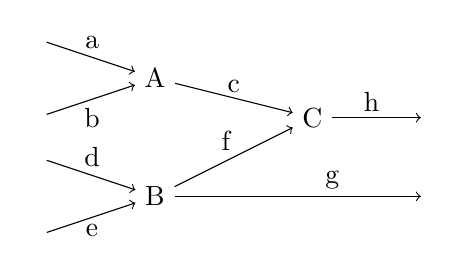
\begin{tikzpicture}
      [scale=.5, auto=center]
      \node (a) at (0,5) {};
      \node (b) at (0,3) {};
      \node (d) at (0,2) {};
      \node (e) at (0,0) {};
      \node (h) at (10,3) {};
      \node (A) at (3,4) {A};
      \node (B) at (3,1) {B};
      \node (C) at (7,3) {C};
      \node (g) at (10,1) {};
      \node (a_1) at (1.4,4.9) {a};
      \node (b_1) at (1.4,3) {b};
      \node (d_1) at (1.4,2) {d};
      \node (e_1) at (1.4,0.14) {e};
      \node (c_1) at (5,3.8) {c};
      \node (f_1) at (4.8,2.4) {f};
      \node (g_1) at (7.5,1.4) {g};
      \node (h_1) at (8.5,3.4) {h};
      \draw[->]
          (a) edge (A) (b) edge (A) (d) edge (B) (e) edge (B) (A) edge (C) (C) edge (h) (B) edge (g) (B) edge (C); 
    \end{tikzpicture}
    \end{center}
    where the "inputs" at each node are covectors and the "outputs" are vectors. Therefore, the entire diagram, which represents the tensor $X$ has a total of 4 inputs (indices $a, b, d, e$) and two outputs (indices $h, g$). We can see from the diagram that the indices $c$ and $f$, which travels "between" the factors are the ones that are being contracted. Therefore, the contraction of $c$ and $f$ contracts the rank (4,6) tensor $A \otimes B \otimes C$ to a rank (2,4) tensor. 
  \end{example}

\subsection{Symmetric and Alternating Tensors}

	Note that $v \otimes w \neq w \otimes v$ in general, but we would like to enforece some symmetry conditions. 

	\begin{definition}[Permutation of Tensor Factors]
	  For some $\sigma \in S_k$, the permutation group, define for an elementary tensor 
		\begin{equation}
			P_\sigma(v_1 \otimes \ldots \otimes v_k) \coloneqq v_{\sigma(1)} \otimes v_{\sigma(2)} \otimes \ldots \otimes v_{\sigma(k)}
		\end{equation}
	\end{definition}

	Note that this is only for elementary tensors, not general tensors. For general tensors, we define the following. 

	\begin{definition}[Symmetric, Alternating Tensors]
		Let $V$ be a vector space over field $\mathbb{F}$ with $\mathrm{char}(\mathbb{F}) \neq k$. Then, for any $T \in V^{\otimes k}$, we define 
		\begin{enumerate}
			\item the \textbf{symmetric component} of $T$ as 
				\begin{equation}
					\Sym: V^{\otimes k} \to V^{\otimes }, \quad \Sym(T) \coloneqq \frac{1}{k!} \sum_{\sigma \in S_k} P_\sigma (T)
				\end{equation}

			\item the \textbf{alternating component} of $T$ as 
				\begin{equation}
					\Alt: V^{\otimes k} \to V^{\otimes }, \quad \Alt(T) \coloneqq \frac{1}{k!} \sum_{\sigma \in S_k} \sgn(\sigma) P_\sigma (T)
				\end{equation}
				where $\sgn(\sigma)$ is the \hyperref[alg-def:signature]{signature} of $\sigma$. 
		\end{enumerate}
	\end{definition}

	Now we would like to find some subspace of tensors that are either symmetric or alternating. 

	\begin{definition}[Symmetric Power]
		The \textbf{kth symmetric power of $V$} of dimension $n$ is the subspace defined in the equivalent ways. 
		\begin{enumerate}
		  \item \textit{Direct Construction}. 
				\begin{equation}
					\Sym^k (V) = \{T \in V^{\otimes k} \colon P_\sigma(T) = T \text{ for all } \sigma \in S_k \}
				\end{equation}

			\item \textit{Quotient Space}. 
				\begin{align}
					\Sym^k (V) = \frac{V^{\otimes k}}{L_{\mathrm{sym}}}, \quad L 
						& = \mathrm{span} \{ T - P_\sigma(T) \colon T \in V^{\otimes k}, \sigma \in S_k \} \\ 
						& = \mathrm{span} \{ v_1 \ldots v_i \otimes v_{i+1} \ldots v_k - v_1 \ldots v_{i+1} \otimes v_i \ldots v_k\}
				\end{align}
		\end{enumerate} 
		We define the symmetric product of elementary tensors as the quotient of the tensor products.
		\begin{equation}
			v_1 \odot \ldots \odot v_n \coloneqq [v_1 \otimes \ldots \otimes v_n] 
		\end{equation}
		which satisfies: 
		\begin{enumerate}
			\item \textit{Symmetric}. $v_1 \ldots v_i \odot \ldots \odot  v_{j} \ldots v_k - v_1 \ldots v_j \odot \ldots \odot v_i \ldots v_k$ for any $1 \leq i \leq j \leq k$. 
			\item \textit{Dimension}. $\dim(\Sym^k (V)) = \binom{n+k-1}{k}$. 
		\end{enumerate}
	\end{definition}
	\begin{proof}
		Let $\Sym^k_1(V)$ be the space defined in (1) and $\Sym^k_2(V)$ be the one defined in (2). Assume that the underlying field has characteristic $0$. Let $\Sym: V^{\otimes k} \to V^{\otimes k}$ be the symmetrization operator on a tensor, defined by
		\begin{equation}
			\Sym(T) = \frac{1}{k!} \sum_{\sigma \in S_k} P_\sigma(T).
		\end{equation}
		We show some facts.
		\begin{enumerate}
			\item \textit{$L_1 = L_2$}. Let us define $L_1$ and $L_2$ as the first and second spans.
				\begin{enumerate}
					\item $L_1 \subseteq L_2$. Given any $T$, we can write it as a linear combination of elementary tensors, so let us work with an elementary tensor $T$ directly. Since \hyperref[alg-thm:transposition_decomposition]{every permutation can be decomposed into adjacent transpositions}, every vector of the form $T - P_\sigma(T)$ can be written as
						\begin{equation}
							\underbrace{T - P_{\tau_1}(T)}_{\in L_2}
							+ \underbrace{P_{\tau_1}(T) - P_{\tau_2}(P_{\tau_1}(T))}_{\in L_2}
							+ \ldots
							+ \underbrace{P_{\tau_{m-1} \cdots \tau_1}(T) - P_{\tau_m \cdots \tau_1}(T)}_{\in L_2},
						\end{equation}
						where $\sigma = \tau_m \cdots \tau_1$ and each $\tau_i$ is an adjacent transposition. This is a linear combination of elements in $L_2$.

					\item $L_2 \subseteq L_1$. Every generator of $L_2$ is of the form
						\begin{equation}
							v_1 \otimes \ldots \otimes v_i \otimes v_{i+1} \otimes \ldots \otimes v_k
							- v_1 \otimes \ldots \otimes v_{i+1} \otimes v_i \otimes \ldots \otimes v_k
							= T - P_{(i,i+1)}(T),
						\end{equation}
						where $P_{(i,i+1)}$ is a transposition, so it is in $L_1$.
				\end{enumerate}
				Therefore, $L_1 = L_2 = L$.

			\item \textit{$\Sym^k_1(V) = \im(\Sym)$}. We first see that for every $\tau \in S_k$,
				\begin{equation}
					P_\tau(\Sym(T))
					= \frac{1}{k!} \sum_{\sigma \in S_k} P_{\tau \sigma}(T)
					= \frac{1}{k!} \sum_{\sigma \in S_k} P_\sigma(T)
					= \Sym(T).
				\end{equation}
				Conversely, if $T$ is symmetric, then
				\begin{equation}
					\Sym(T) = \frac{1}{k!} \sum_{\sigma \in S_k} T = T.
				\end{equation}
				Therefore, we can see that $T \in \im(\Sym) \iff T$ is symmetric $\iff P_\sigma(T) = T$ for all $\sigma \in S_k \iff T \in \Sym^k_1(V)$.

			\item \textit{$\ker(\Sym) = L$}. We prove bidirectionally.
				\begin{enumerate}
					\item $L \subseteq \ker(\Sym)$. $L$ is spanned by terms of the form $T - P_\sigma(T)$. But
						\begin{equation}
							\Sym(T - P_\sigma(T))
							= \frac{1}{k!} \sum_{\gamma \in S_k} \big(P_\gamma(T) - P_{\gamma \sigma}(T)\big)
							= 0
							\implies T - P_\sigma(T) \in \ker(\Sym),
						\end{equation}
						since $\gamma \mapsto \gamma \sigma$ permutes $S_k$.

					\item $\ker(\Sym) \subseteq L$. Let $T \in \ker(\Sym)$. Then,
						\begin{equation}
							T = T - \Sym(T) = \frac{1}{k!} \sum_{\sigma \in S_k} \big(T - P_\sigma(T)\big).
						\end{equation}
						Each summand belongs to $L$, so $T \in L$.
				\end{enumerate}
		\end{enumerate}
		Therefore, by the first isomorphism theorem of vector spaces, we can see that
		\begin{equation}
			\Sym^k_1(V) \simeq \frac{V^{\otimes k}}{\ker(\Sym)}
			= \frac{V^{\otimes k}}{L} = \Sym^k_2(V).
		\end{equation}
		Since this is a quotient space, the relation enforced by the quotient is a congruence relation. Symmetry immediately follows by our quotient definition. For the dimension, let $\{e_1, \ldots, e_n\}$ be a basis of $V$. Then,
		\begin{equation}
			\bigg\{e_1^{\odot a_1} \odot e_2^{\odot a_2} \odot \ldots \odot e_n^{\odot a_n} \colon a_i \geq 0,\; \sum_{i=1}^n a_i = k\bigg\}
		\end{equation}
		is a basis of $\Sym^k(V)$. Indeed, these vectors span $\Sym^k(V)$ since elementary tensors span $V^{\otimes k}$, and they are linearly independent since distinct choices of $(a_1,\ldots,a_n)$ correspond to disjoint sets of elementary basis tensors under symmetrization. By nonnegative stars and bars, we get the dimension
		\begin{equation}
			\dim(\Sym^k(V)) = \binom{n+k-1}{k}.
		\end{equation}
	\end{proof}

	We can clarify this proof by explicitly going through a construction of $\Sym^2(V)$. 

	\begin{example}[Construction of $\Sym^2 (V)$]
		Let $L$ be the subspace of $V \otimes V$ generated by all tensors of the form 
		\begin{equation}
			u \otimes v - v \otimes u, \qquad u, v \in V
		\end{equation}
		For example, given $a, b \in V$ with basis $\{e_1, e_2\}$, 
		\begin{align*}
			a \otimes b - b \otimes a & = (a_1 e_1 + a_2 e_2) \otimes (b_1 e_1 + b_2 e_2) - (b_1 e_1 + b_2 e_2) \otimes (a_1 e_1 + a_2 e_2) \\
			& = (a_1 b_2 - b_2 a_1) e_1 \otimes e_2 + (a_2 b_1 - b_2 a_1) e_2 \otimes e_1 
		\end{align*}

		is an element of $I$. We can generalize this to see that
		\begin{equation}
			\{e_i \otimes e_j - e_j \otimes e_i\}, \; i \neq j
		\end{equation}

		is the basis for $I$. Now, let us define $\Sym^2 V \coloneqq \frac{V \otimes V}{L}$ where, given that $\dim{V} = n$, 
		\begin{equation}
			\dim(\Sym^2 V) = n^2 - \frac{1}{2} n (n-1) = \frac{1}{2} n (n+1)
		\end{equation}

		We denote the elements of $\Sym^2 V$ as $x \odot y$, which are really the equivalence classes $[x \otimes y - y \otimes x]$. Note that
		\begin{align}
			x \odot y - y \odot x & = [x \otimes y - y \otimes x] - [y \otimes x - x \otimes y] \\
														& = [x \otimes y - y \otimes x - y \otimes x + x \otimes y] \\
														& = [0] = 0
		\end{align}

		$\implies x \odot y = y \odot x$. That is, the $\odot$ operator is symmetric, and $\Sym^2 V$ has basis 
		\begin{equation}
			\{e_i \odot e_j\}_{j \geq k}, \quad 1 \leq i \neq j \leq n
		\end{equation}
		which implies that it is invariant under any permutation $p \in S_n$ of the $x_i$'s. 
	\end{example}

	\begin{definition}[Alternating Power]
		The \textbf{kth alternating power of $V$} of dimension $n$ is the subspace defined in the equivalent ways. 
		\begin{enumerate}
		  \item \textit{Direct Construction}. 
				\begin{equation}
					\Sym^k (V) = \{T \in V^{\otimes k} \colon P_\sigma(T) = \sgn(\sigma) T \text{ for all } \sigma \in S_k \}
				\end{equation}

			\item \textit{Quotient Space}. 
				\begin{align}
					\Alt^k (V) = \frac{V^{\otimes k}}{L_{\mathrm{sym}}}, \quad L 
						& = \mathrm{span} \{ T - \sgn(\sigma) P_\sigma(T) \colon T \in V^{\otimes k}, \sigma \in S_k \} \\ 
						& = \mathrm{span} \{ v_1 \ldots v_i \otimes v_{i+1} \ldots v_k + v_1 \ldots v_{i+1} \otimes v_i \ldots v_k\}
				\end{align}
		\end{enumerate}
		We define the \textbf{wedge product} of elementary tensors as the quotient of the tensor products.  
		\begin{equation}
			v_1 \wedge \ldots \wedge v_n \coloneqq [v_1 \otimes \ldots \otimes v_n] 
		\end{equation}
		which satisfies: 
		\begin{enumerate}
			\item \textit{Antisymmetric}. $v_1 \ldots v_i \wedge v_{i+1} \ldots v_k = - v_1 \ldots v_{i+1} \wedge v_i \ldots v_k$. aka, if $v_i = v_j$ for some $i \neq j$, then $v_1 \ldots v_i \wedge v_{i+1} \ldots v_k = 0$. 
			\item \textit{Dimension}. $\dim(\Sym^k (V)) = \binom{n}{k}$. 
		\end{enumerate}
	\end{definition}
	\begin{proof}
		Let $\Alt^k_1(V)$ be the space defined in (1) and $\Alt^k_2(V)$ be the one defined in (2). Assume that the underlying field has characteristic $0$. Let $\Alt: V^{\otimes k} \to V^{\otimes k}$ be the antisymmetrization operator on a tensor, defined by
		\begin{equation}
			\Alt(T) = \frac{1}{k!} \sum_{\sigma \in S_k} \sgn(\sigma) P_\sigma(T).
		\end{equation}
		We show some facts.
		\begin{enumerate}
			\item \textit{$L_1 = L_2$}. Let us define $L_1$ and $L_2$ as the first and second spans.
				\begin{enumerate}
					\item $L_1 \subseteq L_2$. Given any $T$, we can write it as a linear combination of elementary tensors, so let us work with an elementary tensor $T$ directly. Since \hyperref[alg-thm:transposition_decomposition]{every permutation can be decomposed into adjacent transpositions}, every vector of the form $T - \sgn(\sigma) P_\sigma(T)$ can be written as
						\begin{align}
							&\underbrace{T + P_{\tau_1}(T)}_{\in L_2}
							- \underbrace{\big(P_{\tau_1}(T) + P_{\tau_2}(P_{\tau_1}(T))\big)}_{\in L_2}
							+ \ldots \notag\\
							&\qquad + (-1)^{m-1}
							\underbrace{\big(P_{\tau_{m-1}\cdots\tau_1}(T)
							+ P_{\tau_m\cdots\tau_1}(T)\big)}_{\in L_2},
						\end{align}
						where $\sigma = \tau_m \cdots \tau_1$ and each $\tau_i$ is an adjacent transposition. This is a linear combination of elements in $L_2$.

					\item $L_2 \subseteq L_1$. Every generator of $L_2$ is of the form
						\begin{equation}
							v_1 \otimes \ldots \otimes v_i \otimes v_{i+1} \otimes \ldots \otimes v_k
							+ v_1 \otimes \ldots \otimes v_{i+1} \otimes v_i \otimes \ldots \otimes v_k
							= T + P_{(i,i+1)}(T),
						\end{equation}
						where $P_{(i,i+1)}$ is a transposition, so $\sgn((i,i+1))=-1$ and it is in $L_1$.
				\end{enumerate}
				Therefore, $L_1 = L_2 = L$.

			\item \textit{$\Alt^k_1(V) = \im(\Alt)$}. We first see that for every $\tau \in S_k$,
				\begin{align}
					P_\tau(\Alt(T))
					&= \frac{1}{k!} \sum_{\sigma \in S_k} \sgn(\sigma) P_{\tau\sigma}(T)\\
					&= \frac{\sgn(\tau)}{k!} \sum_{\sigma \in S_k} \sgn(\tau\sigma) P_{\tau\sigma}(T)\\
					&= \sgn(\tau)\Alt(T).
				\end{align}
				Conversely, if $T$ is alternating, then
				\begin{equation}
					\Alt(T) = \frac{1}{k!} \sum_{\sigma \in S_k} \sgn(\sigma)^2 T = T.
				\end{equation}
				Therefore, we can see that $T \in \im(\Alt) \iff T$ is alternating $\iff P_\sigma(T) = \sgn(\sigma)T$ for all $\sigma \in S_k \iff T \in \Alt^k_1(V)$.

			\item \textit{$\ker(\Alt) = L$}. We prove bidirectionally.
				\begin{enumerate}
					\item $L \subseteq \ker(\Alt)$. $L$ is spanned by terms of the form $T - \sgn(\sigma)P_\sigma(T)$. But
						\begin{align}
							&\Alt(T - \sgn(\sigma)P_\sigma(T))\\
							&\quad = \frac{1}{k!}\sum_{\gamma \in S_k}
							\big(\sgn(\gamma)P_\gamma(T)
							- \sgn(\gamma)\sgn(\sigma)P_{\gamma\sigma}(T)\big)\\
							&\quad = 0,
						\end{align}
						since $\gamma \mapsto \gamma\sigma$ permutes $S_k$ and $\sgn(\gamma)\sgn(\sigma)=\sgn(\gamma\sigma)$. Therefore, $T - \sgn(\sigma)P_\sigma(T) \in \ker(\Alt)$.

					\item $\ker(\Alt) \subseteq L$. Let $T \in \ker(\Alt)$. Then,
						\begin{equation}
							T = T - \Alt(T) = \frac{1}{k!}\sum_{\sigma \in S_k}
							\big(T - \sgn(\sigma)P_\sigma(T)\big).
						\end{equation}
						Each summand belongs to $L$, so $T \in L$.
				\end{enumerate}
		\end{enumerate}
		Therefore, by the first isomorphism theorem of vector spaces, we can see that
		\begin{equation}
			\Alt^k_1(V) \simeq \frac{V^{\otimes k}}{\ker(\Alt)}
			= \frac{V^{\otimes k}}{L} = \Alt^k_2(V).
		\end{equation}
		Since this is a quotient space, the relation enforced by the quotient is a congruence relation. Antisymmetry immediately follows by our quotient definition. In particular, if $v_i = v_j$ for some $i \neq j$, then
		\begin{equation}
			v_1 \wedge \ldots \wedge v_k
			= -v_1 \wedge \ldots \wedge v_k = 0.
		\end{equation}
		For the dimension, let $\{e_1,\ldots,e_n\}$ be a basis of $V$. Then,
		\begin{equation}
			\big\{e_{i_1} \wedge \ldots \wedge e_{i_k}
			\colon 1 \leq i_1 < \ldots < i_k \leq n\big\}
		\end{equation}
		is a basis of $\Alt^k(V)$. Indeed, these vectors span $\Alt^k(V)$ since elementary tensors span $V^{\otimes k}$, and they are linearly independent since distinct choices of $(i_1,\ldots,i_k)$ correspond to disjoint sets of elementary basis tensors under antisymmetrization. By choosing $k$ distinct indices from $n$, we get the dimension
		\begin{equation}
			\dim(\Alt^k(V)) = \binom{n}{k}.
		\end{equation}
	\end{proof}

	\begin{example}[Inner Product]
    The inner product $\langle \cdot, \cdot \rangle$ on $V$ is an element of $\Sym^2 V$, since it is a bilinear, symmetric operation on $V$. 
  \end{example}

	\begin{example}[$\Sym^2 (V)$ is Symmetric Matrices]
		One realization of $\Sym^2 \mathbb{R}^n$ is the set of all symmetric $n \times n$ real matrices. 
	\end{example}

	\begin{example}[$\Alt^2(V)$ is Antisymmetric Matrices]
    Let $I$ be a subspace of $V \otimes V$ generated by elements of the form $x \otimes x \in V \otimes V$. That is, given a basis $\{e_i\}$ of $n$-dimensional space $V$, all tensors of the form $x \otimes x \in V \otimes V$ can be written 
		\begin{equation}
    	x \otimes x = \sum_{i=1}^n a_i (e_i \otimes e_i) + \sum_{i \neq j} b_{i j} (e_i \otimes e_j + e_j \otimes e_i)
		\end{equation}
    which implies that the components of $e_i \otimes e_j$ and $e_j \otimes e_i$ must be the same for every element in $I$. Since we can group the components $e_i \otimes e_j$ and $e_j \otimes e_i$ together to $e_i \otimes e_j + e_j \otimes e_i$, the basis of $I$ is 
		\begin{equation}
			\{e_1 \otimes e_1, \cdots, e_n \otimes e_n, e_1 \otimes e_2 + e_2 \otimes e_1, \cdots, e_{n-1} \otimes e_n + e_n \otimes e_{n-1}\}
		\end{equation}
		One realization of the space $\Lambda^2 \mathbb{R}^n$ is the set of antisymmetric $n \times n$ matrices. 
	\end{example}

	\begin{example}[Third Exterior Power]
		For $n = 3$ (and assuming that $\dim{V} \geq 3$), the subspace $I \subset V \otimes V \otimes V$ is the space generated by elements of the forms $\{x \otimes x \otimes y, x \otimes y \otimes x, y \otimes x \otimes x\}$. Following a similar construction, the \textbf{third exterior power of $V$} is
		\begin{equation}
			\Lambda^3 V \coloneqq \frac{V \otimes V \otimes V}{I}
		\end{equation}
		with its elements being equivalence classes of the form
		\begin{equation}
			x \wedge y \wedge z,\; x, y, z \in V
		\end{equation}
		such that
		\begin{align*}
			x \wedge y \wedge z & = - x \wedge z \wedge y \\
			& = - y \wedge x \wedge z \\
			& = - z \wedge y \wedge x
		\end{align*}
		The basis of $\Lambda^3 V$ is
		\begin{equation}
			\{e_i \wedge e_j \wedge e_k \; | \; i < j < k\} \implies \dim{\Lambda^3 V} = \frac{1}{6} n (n-1) (n-2)
		\end{equation}
	\end{example}

	\begin{example}[Cross Product]
    Given 3 dimensional vector space $V$ with basis $\{e_1, e_2, e_3\}$, the wedge product of two vectors $a, b \in V$ is 
    \begin{align}
      a \wedge b & = (a_1 e_1 + a_2 e_2 + a_3 e_3) \wedge (b_1 e_1 + b_2 e_2 + b_3 e_3) \\
      & = (a_2 b_3 - a_3 b_2) e_2 \wedge e_3 + (a_3 b_1 - a_1 b_3) e_3 \wedge e_1 + (a_1 b_2 - a_2 b_1) e_1 \wedge e_2 
    \end{align}
    which is essentially the formula for the cross product $\times$ in Euclidean space. We can therefore think of the realization of the wedge product in 3 dimensional space $V$ as the cross product. 
		\begin{equation}
    	\wedge: V \times V \longrightarrow \Lambda^2 V
		\end{equation}
    Note that $\Lambda^2 V \simeq V$ if $\dim{V} = 3$, so we can construct the more familiar $\times$ operation in $\mathbb{R}^3$. 
		\begin{equation}
    	\times: \mathbb{R}^3 \times \mathbb{R}^3 \longrightarrow \Lambda^2 \mathbb{R}^3 \simeq \mathbb{R}^3
		\end{equation}
    which is consistent with $\times$ taking two vectors and outputting a third vector living in $\mathbb{R}^3$ that is orthogonal to the two input vectors. 
  \end{example}

	\begin{example}[Triple Scalar Product]
    The realization of the wedge product of 3 vectors in 3 dimensional space $V$ is the \textit{triple scalar product}, which we will denote as $\times_3$
		\begin{equation}
    	\wedge: V \times V \times V \longrightarrow \Lambda^3 V
		\end{equation}
    Note that since $\Lambda^3 V \simeq V$ when $\dim{V} = 3$, we can write 
		\begin{equation}
    	\times_3: \mathbb{R}^3 \times \mathbb{R}^3 \times \mathbb{R}^3 \longrightarrow \Lambda^3 \mathbb{R}^3 \simeq \mathbb{R}
		\end{equation}
    which is consistent with $\times_3$ taking three vectors and outputting the signed volume of their parallelopiped which lies in $\mathbb{R}$. 
  \end{example}

	\begin{definition}[Determinant]
		The \textbf{determinant} of a linear map $A: V \to V$ is the singular basis vector\footnote{Note that any tensor in $\Lambda^n V$ satisfies multilinearity and antisymmetricity, but only the basis vector $e_1 \wedge \cdots \wedge e_n$ satisfies the normalizing condition $\det{I} = 1$. Since, given that the dual basis of $V^*$ is $\{f_j\}$, $(e_1 \wedge \cdots \wedge e_n) (f_1, f_2, \cdots, f_n) = \prod_{i=1}^n e_i (f_i) = \prod_{i=1}^n \delta_i^i = 1$. } of the $1$-dimensional space $\Lambda^n (V)$. 
		\begin{equation}
    	e_1 \wedge e_2 \wedge \cdots \wedge e_{n-1} \wedge e_n
		\end{equation}
  \end{definition}

	Note that this construction of the determinant is consistent with our previous construction of the determinant of a matrix since $e_1 \wedge \cdots \wedge e_n$ is indeed multilinear and antisymmetric. In its purest sense, 
	\begin{equation}
		e_1 \wedge \cdots \wedge e_n: \prod_{i=1}^n V^* \longrightarrow \mathbb{F}
	\end{equation}
	is a mapping that is multilinear and antisymmetric. But there is an inconsistency. The matrix determinant takes in \textit{matrices} rather than taking in $n$-tuples of covectors. However, we can interpret the $n$ covectors in $V^* \times \cdots \times V^*$ as the column (or row) vectors of an $n \times n$ matrix. This completes the realization, and so we can conclude that the matrix determinant is just a realization of the more abstract determinant $e_1 \wedge \cdots \wedge e_n$. 

  There is a simple relationship between $V \otimes V$, $\Lambda^2 V$, and $\Sym^2 V$. 

	\begin{theorem}[Symmetric-Antisymmetric Decomposition]
    We can always factor a rank (2,0) tensor into its symmetric and antisymmetric parts. In fact, 
		\begin{equation}
    	V \otimes V \simeq \Sym^2 V \oplus \Lambda^2 V
		\end{equation}
    with isomorphism defined
		\begin{equation}
    	v \otimes w \mapsto \Big( \frac{1}{2} (v \odot w), \frac{1}{2} (v \wedge w) \Big)
		\end{equation}
  \end{theorem}
  \begin{proof}
    Given $v \otimes w \in V \otimes V$, 
		\begin{equation}
    	v \otimes w + w \otimes v \in \Sym^2 V \text{ and } v \otimes w - w \otimes v \in \Lambda^2 V
		\end{equation}
    By defining $v \odot w$ and $v \wedge w$ as the expressions above, the isomorphism is satisfied. 
  \end{proof}

  Therefore, when working in $V \otimes V$, we can interpret 
  \begin{align}
		v \wedge w & = \frac{1}{2} (v \otimes w - w \otimes v) \\
		v \odot w & = \frac{1}{2} (v \otimes w + w \otimes v) 
  \end{align}

  However, $V \otimes V \otimes V \not\simeq \Sym^3 V \oplus \Lambda^3 V$. \textit{Schur functors} are used to fix this discrepancy. 

\subsection{Tensor Algebras}

	We would like to ``add'' differently ranked tensors together. In order to do so, we can just construct a bigger vector space as the direct sum of all of the higher order tensor product spaces. 

	\begin{definition}[Tensor Algebra]
    The \textbf{tensor algebra} of vector space $V$ over field $\mathbb{F}$ is an associative, noncommutative algebra defined
    \begin{align}
      T(V) \coloneqq \bigoplus_{n = 0}^{\infty} V^{\otimes n} & = V^{\otimes 0} \oplus V^{\otimes 1} \oplus V^{\otimes 2} \oplus V^{\otimes 3} \oplus \cdots \\
      & = \mathbb{F} \oplus V \oplus V^{\otimes 2} \oplus V^{\otimes 3} \oplus V^{\otimes 4} \oplus\cdots 
    \end{align}
    with elements being infinite-tuples
		\begin{equation}
    	(a, B^\mu, C^{\nu \gamma}, D^{\alpha \beta \epsilon}, \cdots)
		\end{equation}
    The addition operation is defined component-wise, and the multiplication operation is the tensor product 
		\begin{equation}
    	\otimes: T(V) \times T(V) \longrightarrow T(V)
		\end{equation}
    and the identity element is
		\begin{equation}
    	I = (1, 0, 0, \cdots)
		\end{equation}
  \end{definition}
	\begin{proof}
    Linearity is easily proved. In order to do this rigorously, we must define the map (which is also an isomorphism)
		\begin{equation}
			i_j: V^{\otimes j} \longrightarrow T(V), \; i_j (T^{\kappa_1, \cdots, \kappa j}) = (0, \cdots,0, T^{\kappa_1, \cdots, \kappa j}, 0, \cdots, 0)
		\end{equation}
		So, we can implicitly define the addition of arbitrary tensors $A \in V^{\otimes n}$ and $B \in V^{\otimes m}$ as 
		\begin{equation}
			A + B \coloneqq i_n (A) + i_m (B) \in T(V)
		\end{equation}
		along with the tensor multiplication of the form
		\begin{equation}
			A \otimes B \coloneqq i_n(A) \otimes i_m(B) \coloneqq i_{n+m} (A \otimes B)
		\end{equation}
		This allows us to alternatively define the tensor product operation as
		\begin{equation}
			i_i(V^{\otimes i}) \otimes i_j( V^{\otimes j}) \coloneqq i_{i+j} (V^{\otimes (i+j)})
		\end{equation}
	\end{proof}

	\begin{definition}[Symmetric Algebra]
    The \textbf{symmetric algebra} of vector space $V$ of dimension $n$ is defined
		\begin{equation}
    	\Sym (V) \coloneqq \bigoplus_{k=0}^\infty \Sym^k V
		\end{equation}
		where $\Sym^0 (V) = \mathbb{F}$. It is infinite-dimensional. 
  \end{definition}

	\begin{definition}[Exterior Algebra]
    The \textbf{symmetric algebra} of vector space $V$ of dimension $n$ is defined
		\begin{equation}
			\Alt(V) \coloneqq \bigoplus_{k=0}^n \Alt^k V \coloneqq \Alt^0 V \oplus \Alt^1 V \oplus \Alt^2 V \oplus \cdots \oplus \Alt^n V 
		\end{equation}
		where $\Alt^0 (V) = \mathbb{F}$. It has dimension $2^n$. 
	\end{definition}

